\documentclass[12pt]{article}

\usepackage{graphicx}
\usepackage{svg}

\newcommand{\code}[1]{\texttt{#1}}

\usepackage[utf8]{inputenc}
\usepackage[
    twoside,
    top=1in,
    bottom=0.75in,
    inner=0.5in,
    outer=0.5in
]{geometry}

\usepackage{tcolorbox}
\tcbuselibrary{skins}
\usepackage{minted}
\usepackage{color}
\usepackage{tikz}
\usetikzlibrary{calc}
\usepackage{tabularx,colortbl}
\usepackage{amsfonts,amsmath,amssymb}
\usepackage{titling}
\usepackage{mathrsfs}
\usepackage{calc}
\usepackage{graphicx}
\usepackage{svg}
\usepackage[
    backend=biber,
    style=authoryear,
    sorting=nyt
]{biblatex}

\addbibresource{bibliography.bib}


\title{Homework Template and Samples}
\author{Heather Tweedie}
\date{March 2023}

\linespread{1.25}

\begin{document}

%%%% Format Running Header %%%%%
\markboth{\theauthor}{\thetitle}

%%%% Insert the Title Information %%%
\maketitle


%%%% General Description of the Document %%%%
\begin{abstract}

\end{abstract}

\section{Introduction}

The threats posed by climate change brought about primarily by increases in anthropogenic emissions means it is necessary to develop
models that are capable of predicting the impacts of these changes. The models used to predict long-term future climate variations
are similar to those used to model present weather and climate conditions (Raäisaänen, 2007), and as such, it is important that these
models are well-understood.

This study aims to determine if the weather and climate at a location can be predicted using basic machine learning techniques. Two
main research questions are proposed:

\begin{enumerate}
  \item How accurately can a model predict the climate of a location a year in advance?
  \item Can a model predict the weather at a location any better than assuming the weather tomorrow will be the same as the weather today?
\end{enumerate}

\section{Data used}

The data used in this study were obtained from the Global Historical Climate Network (GHCN). GHCN-Daily (GHCND) (Menne et al., 2012a)
is a database of daily weather summaries featuring data from over 80,000 stations in 180 countries (Menne et al., 2012). Approximately
two thirds of the stations report precipitation data only, however many stations report maximum and minimum temperatures, snowfall and
depth in addition. The data come from a number of global sources including the National Oceanic and Atmospheric Administration, the
European Climate Assessment and Dataset, and the South African Weather Service, and are subjected to automated, unsupervised quality
assurance tests.

Only stations which are part of the GCOS Surface Network (GSN) were included in this study. As of March 2019, 1023 stations were part 
of this network (Oakley, 2018), providing an approximately uniform coverage of the globe with high-quality data of a good length 
(GCOS, n.d.) (Figure 1).

    \begin{figure}
        \centering
        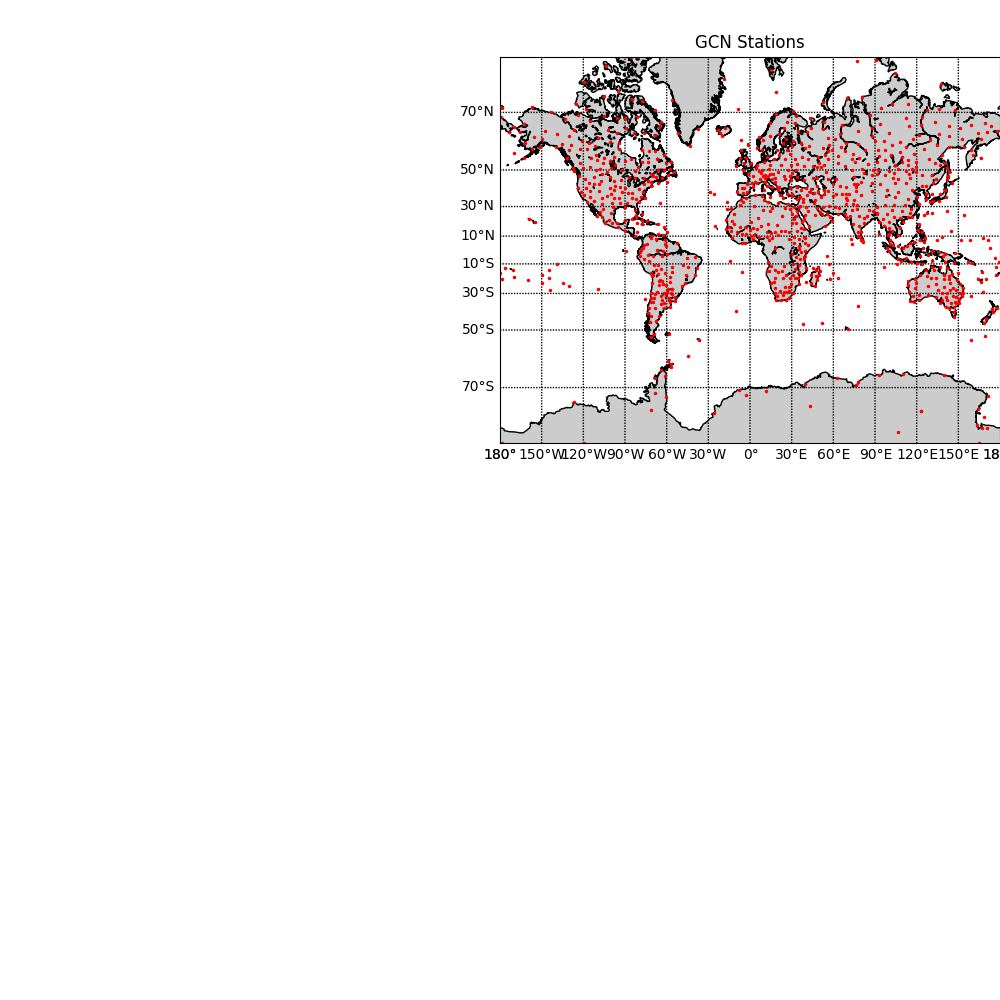
\includegraphics[scale = 1.2]{all_stations.png}
        \caption{All stations included in the GCOS Surface Network (GSN). Stations are marked as red points and plotted on a basemap 
        of the Mercator projection. The network provides a relatively uniform coverage of global land areas.}
        \label{fig:my_label}
    \end{figure}

\section{Predicting the weather}
\subsection{Methodology}


To further filter the stations used, the number of missing data points from the variables in question were counted; the stations with 
no or fewer than 100 gaps were focused upon for study. A station to investigate was selected on this basis, and the data for that 
station acquired from a course-provided directory of GSN station data files. Time-series data for the specified variables were then 
extracted from this file and stored in separate instances of the `Variable` class with fields for the values and their corresponding 
dates. The dates were converted from their original ‘DateTime’ format, to the number of days since the first observation.

At this point, the data were normalised, bringing them all to a similar scale which will improve the performance and stability of the
 model during training. This was carried out by subtracting the mean of the entire dataset, then dividing by the maximum value found 
 in that set. Figure [x] shows the first ten months of climate data for station [x] as both the mean monthly values and the normalised
  mean values.

Following normalisation, the data were concatenated from individual 1-d arrays into a single n-d array, then subdivided into training, 
validation and testing datasets. There were a number of considerations to make when deciding on ratios for these datasets. The training
 dataset must be sufficiently large to prevent high variance during training of the model, but the validation and testing datasets must 
 be large enough to prevent high variance when evaluating the model. The validation dataset is used to tune the hyperparameters of the 
 model, and given that in this case there are relatively few of these, a smaller dataset is used. A final training to testing to validation 
 ratio of 0.7 : 0.2 : 0.1 is implemented.

The divided datasets were then split into a series of overlapping windows, with lengths equal to the defined window size, and an associated 
value a number of data points ahead in the time series, dictated by the defined offset. These are the input windows and targets on which the 
model will be trained, validated and tested. These windows are reshaped from (number of windows, window size) to (number of windows, window 
size, number of features), where ‘number of features’ is the number of variables being used in this model’s training, in this case, two.

The model to be trained on the input data described above employs layers of long short-term memory, as described by Hochreiter and Schmidhuber (1997).

\subsection{Results}

\section{Predicting the climate}

\subsection{Methodology}

To prepare the data for investigating climate prediction, the mean values for each month of data were calculated. The data for both the climate
 and weather prediction models were at this point normalised. This brings all the data to a similar scale, improving the performance and 
 stability during training of the model. The data were normalised by subtracting the mean of the entire dataset, then dividing by the maximum 
 value found in that set. Figure [x] shows the first ten months of climate data for station [x] as both the mean monthly values and the 
 normalised mean values.

Following normalisation, the data were divided into training, validation and testing datasets. The training dataset must be sufficiently 
large to prevent high variance during training of the model, but the validation and testing datasets must be large enough to prevent high 
variance when evaluating the model. The validation dataset is used to tune the hyperparameters of the model, and given that in this case 
there are relatively few of these, a smaller dataset is used. A final training to testing to validation ratio of 0.7 : 0.2 : 0.1 is implemented.

In the case of the climate model, an offset of 12 is used, meaning the model will predict twelve months ahead. The window size dictates much data 
the model is trained on in a single batch. If this is too small, the model will not perform well as it will not have been trained on sufficiently 
long sequences , however if it is too large, the training will take a long time to run and the model may overfit the data. The window size must
 also be smaller than the validation dataset minus the offset, otherwise it is impossible to shape the daraser as necessary during later steps. 
 It was found during testing that a window size of 80 worked well and gave good performance. A check was also included to reduce this window size
  for any dataset in which this window size would be too large for the size of the validation set.

The divided datasets were then split into a series of overlapping windows, with lengths equal to the defined window size, and an associated value
 a number of data points ahead in the time series, dictated by the defined offset. These are the input windows and targets on which the model will
  be trained, validated and tested. These windows are reshaped from (number of windows, window size) to (number of windows, window size, number 
  of features), where ‘number of features’ is the number of variables being used in this model’s training, in this case, one.

\subsection{Results}
\end{document}
